
\documentclass[twocolumn,11pt]{article}
\setlength{\textheight}{9truein}
\setlength{\topmargin}{-0.9truein}
\setlength{\parindent}{0pt}
\setlength{\parskip}{10pt}
\setlength{\columnsep}{.4in}
\newcommand{\beq}{\begin{equation}}
\newcommand{\eeq}{\end{equation}}
\renewcommand{\abstractname}{Abstract}
\usepackage{graphicx}
\usepackage{url}
\title{NAEST - Experiment 03 Report \\  Exploring Light Refraction and Total Internal Reflection: An Experimental Study Using a Water Box Prism}
\author{Shuvam Banerji Seal\\2023WB00609}
\date{\today}
\usepackage{ragged2e}
\usepackage{amsmath}

\usepackage{textcomp}
\usepackage{siunitx}

\usepackage{mathtools}
\newtagform{dots}{\ldots(}{)}
\usepackage{amsfonts}
\usepackage{caption}
\usepackage{stackengine}
\usepackage{amssymb}
\usepackage{graphicx}
\usepackage{accents}
\usepackage{booktabs}
\usepackage{eqnarray}
\usepackage{url}
\usepackage{blindtext}
\usepackage{tcolorbox}
\usepackage{graphicx}   
\usepackage{amsthm}
\usepackage{algorithm}
\usepackage{hyperref}
\hypersetup{
    colorlinks=true,
    linkcolor=blue,
    filecolor=magenta,      
    urlcolor=blue,
    pdftitle={NAEST-Shuvam Banerji Seal},
    pdfpagemode=FullScreen,
    }
\usepackage{gensymb}
\usepackage{algpseudocode}
\usepackage{subcaption}
\usepackage[english]{babel}
\usepackage[export]{adjustbox}
\usepackage{enumerate}
\usepackage[left=2.5cm,right=2.5cm,top=1.5cm,bottom=1.5cm]{geometry}
\usepackage{lineno}
\usepackage{cite}
\usepackage{acronym}
\usepackage{xcolor}
\newcommand{\remark}[3]{%
    {\colorbox{#2}{\sffamily\scriptsize\bfseries\textcolor{white}{#1}}}
    {\sffamily\small\itshape\textcolor{#2}{#3}}
}

\begin{document}
\definecolor{aqua}{rgb}{0.0, 1.0, 1.0}
%\hypersetup{colorlinks,urlcolor=blue}
\pagestyle{plain}
 \twocolumn[
   \begin{@twocolumnfalse}
   \textbf{\maketitle}
   \setlength{\parindent}{0pt}
   \begin{abstract} 
   \textbf{Keywords:} light refraction, total internal reflection, water box prism, refractive index, critical angle, optical phenomena, self-constructed apparatus, angle measurement, data analysis, optical properties, light-matter interaction, experimental study, error analysis.\\
\vspace{0.5cm}
\\
This experimental study investigates light refraction and total internal reflection phenomena using a self-constructed water box prism. The setup includes a rectangular transparent plastic box, a cardboard sheet, and a mobile torch. By manipulating angles and analyzing data, we explore these optical behaviors. We measure the refractive index of water using minimum deviation and critical angle methods, obtaining values of $\mu_{water} = 1.306$ and $\mu_{water} = 1.346$, respectively. Additionally, we observe total internal reflection with a calculated critical angle of $48\degree$. Discrepancies in the prism angle are analyzed, revealing a value of $A_{real} = 98\degree$. The refractive index of saltwater is measured as $\mu_{salt_{water}} = 1.49$. Sources of error, including instrumental and human factors, are discussed. This experiment provides practical insights into light-matter interactions and optical principles.

		\vspace{.3in} 
     \end{abstract}
    \end{@twocolumnfalse}]



\section{Introduction}
The captivating dance of light has intrigued scientists and thinkers for centuries, unlocking secrets of the natural world. In this experiment, we embark on a journey to explore the mesmerizing phenomena of light refraction and total internal reflection using a novel tool – a self-constructed water box prism. By harnessing readily available materials, we unveil the captivating interactions between light and matter that lie within our grasp.

With a scientific spirit, we set the stage for experimentation. Armed with a rectangular transparent plastic box, a humble cardboard sheet, and a mobile torch, we orchestrate a symphony of light and water. As we manipulate angles and observe colours, we unravel the mysteries surrounding us.

As we journey through this experiment, we gain insights into the properties of light and engage in critical thinking and data analysis. We challenge assumptions, scrutinize measurements, and embrace the intricacies of scientific exploration.

Join us as we peer through the prism of curiosity, where light and water converge to reveal the magic that lies beneath the surface. Let the experiment unfold, and the secrets of light unveil themselves before our eager eyes.

Welcome to the realm of light refraction and total internal reflection – a realm where ordinary materials illuminate the extraordinary wonders of the universe\footnote{I don't know why I wrote it like the beginning of a science fiction book}.
\section{Aim:}
Our aim is twofold: 
\begin{enumerate}
    \item to measure the refractive index of water, a fundamental property that dictates how light bends as it transitions from one medium to another.
    \item we delve into the enigmatic realm of total internal reflection, an awe-inspiring phenomenon where light seemingly defies its own rules.
\end{enumerate} 

\section{Materials Required}
\begin{itemize}
    \item Rectangular transparent plastic box with a flat base\footnote{This was very difficult to find. Finally, I did get one with minimum amount of interfering designs.}
    \item Cardboard sheet
    \item Mobile torch \footnote{And the smartphone is also important for taking snapshots of the experiment. Also it is an important measuring tool.}
    \item Paper for observing light beams
    \item Water
    \item Salt/sugar (for extra exploration)
    \item Ruler
    \item Protractor\footnote{I searched for it from almost everyone but couldn't find one. Maybe college students have forgotten about it. Now, why I didn't just buy one? Interestingly, it was not available from the on-campus stationary shop and I just didn't want to go to the outside shops(too far...2km). And maybe because it's easier to get the angle from pictures taken parallel to the surface of the experiment. }
    \item Adhesive tape (to hold cardboard slit)\footnote{I used books}
    \item Pen/pencil for marking
    \item Optional: Second cardboard sheet for parallel beam setup
\end{itemize}

\section{Procedure}

\subsection{Part 1: Refractive Index of Water}
\begin{enumerate}
    \item Set up the apparatus as described in the "Setting up the Apparatus" section of the provided problem sketch.
    \begin{figure}[H]
        \centering
        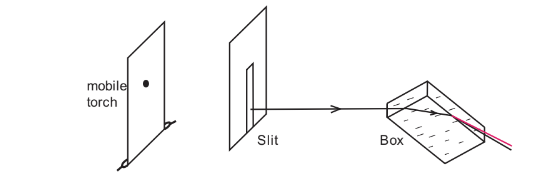
\includegraphics[scale =0.5]{deviation_illustration.png}
        \caption{Illustration of the Experimental procedure}
        \label{Illustration of the Experimental procedure}
    \end{figure}
    % ... Continue with the rest of the steps in Part 1 ...
    
    \item Calculate the refractive index of water using the given formula.
    
    \begin{equation}
        \label{Deviationoflight}
        \mu_{water} = \frac{\sin{\frac{\delta_{min} + A}{2}}}{\sin{\frac{A}{2}}} 
    \end{equation}
\end{enumerate}

\subsection{Part 1 (b): Total Internal Reflection}
\begin{enumerate}
    \item Rotate the box to achieve total internal reflection and measure the angle of incidence ($i$).
    
    % ... Continue with the rest of the steps in Part 1 (b) ...
\end{enumerate}

\subsection{Part 2: Discrepancies in the Angle of Prism}
\begin{enumerate}
    \item Set up parallel beams of light using two torches and slits, as detailed in the "Setting up Parallel Beams" section. \footnote{In reality, two sources were creating difficulty due to them being close. As the slits were not far apart, I used the same source for better results.}
        \begin{figure}[H]
        \centering
        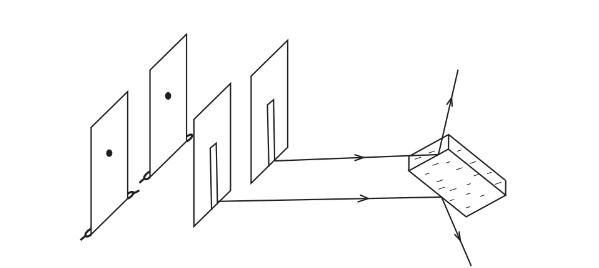
\includegraphics[scale =0.5]{Given setup for tir.png}
        \caption{Expected setup for Discrepancies in the Angle of Prism}
        \label{Illustration of the Experimental procedure}
    \end{figure}

    
    % ... Continue with the rest of the steps in Part 2 ...
\end{enumerate}

\subsection{Extra Exploration: Experiment with Salt/Sugar Water}
\begin{enumerate}
    \item Prepare salt/sugar water and fill the plastic box.
    \item Repeating the same steps
    
    % ... Continue with the steps for the extra exploration ...
\end{enumerate}

\section{Observations, Data Tabulation and Calculations}

\subsection{Part 1.a: Estimating the Refractive Index of Water using the Deviation of Light through a Water prism concept }
   I have used Photoshop editing software to get the angle based on the colour spectrum by selecting the one with some red gradations and also special care was given to level the photograph parallel to the surface of the set-up using the gyroscope of the smartphone during the capturing of the snapshot.
    
    
    \begin{figure}[H]
        \centering
        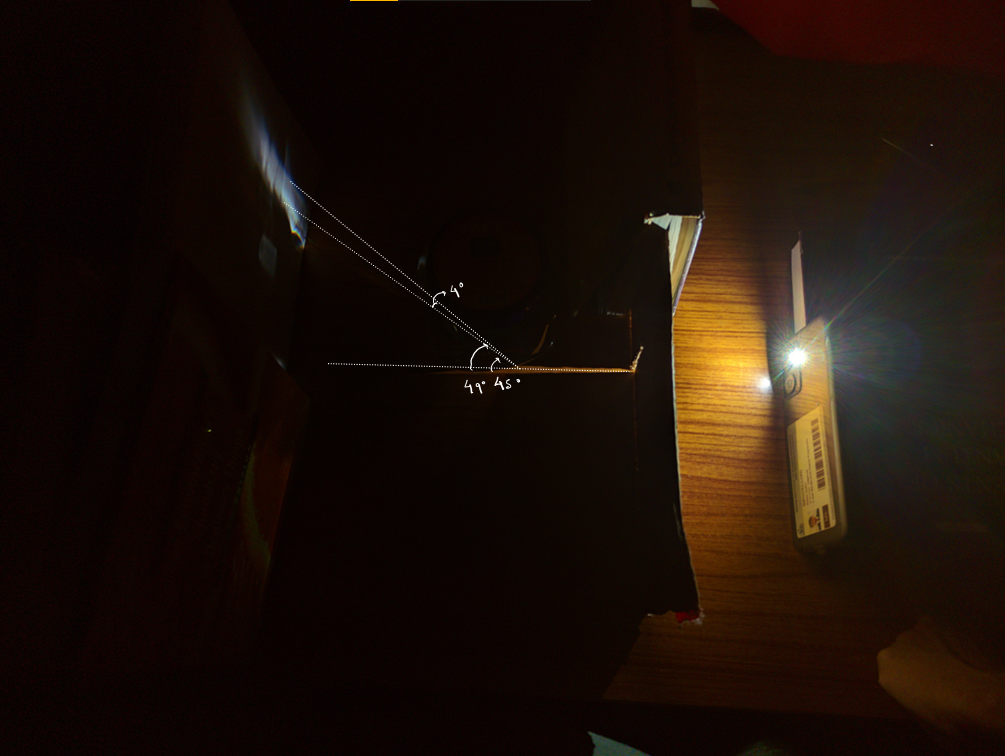
\includegraphics[scale =0.3]{red_violet.png}
        \caption{The given snapshot shows the deviation of the incident light beam. I tried to select the red colour from the spectrum to get the minimum angle of deviation. Click \href{https://drive.google.com/drive/folders/1kRDKGAJyG9_05VehqO_25z_MpxRcHcj9?usp=drive_link}{here} for the raw pictures.}
        \label{Angle of deviation _45}
    \end{figure}
From the picture we get,
\begin{equation}
    \label{deviation value for single setup}
    \delta_{min} = 45 \degree
\end{equation}
\subsubsection{Calculations:}
Putting the value of $\delta_{min}$ from \eqref{deviation value for single setup} in \eqref{Deviationoflight}, and as per the given instructions, setting the prism angle to $A = 90\degree$ we get,
\begin{equation}
    \label{Refractive Index from single setup}
    \mu_{water} = 1.306
\end{equation}

\subsection{Extra-Calculations:}
\subsubsection{Measuring the Real angle of the Prism and calculations:}

I used the same methodologies to get the prism angle.
Now using this we get,
\begin{equation}
    \label{Refractive Index from single setup_real prism}
    {\mu_{water_}}_{A=98\degree} = 1.26
\end{equation}

We will later confirm this angle of prism in the part-2 of this experiment.
    \begin{figure}[H]
        \centering
        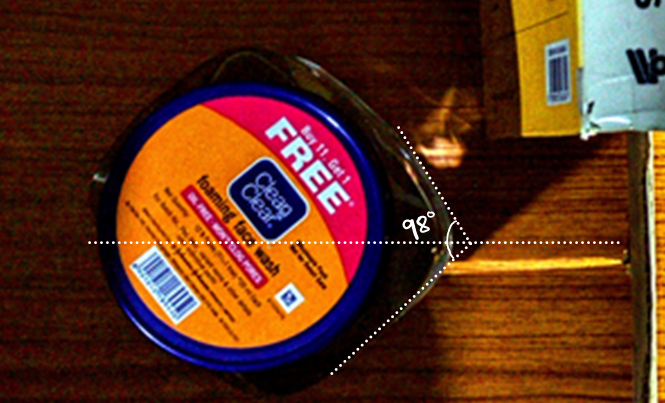
\includegraphics[scale =0.45]{prism_real_angle.png}
        \caption{The real angle of the Prism comes out to be $98\degree $}
        \label{Real angle of the prism}
    \end{figure}

\subsubsection{Estimating the Refractive Indices with respect to red and blue light}
Refer figure \eqref{Angle of deviation _45}, for the data used,

\begin{comment}
        \begin{figure}[H]
        \centering
        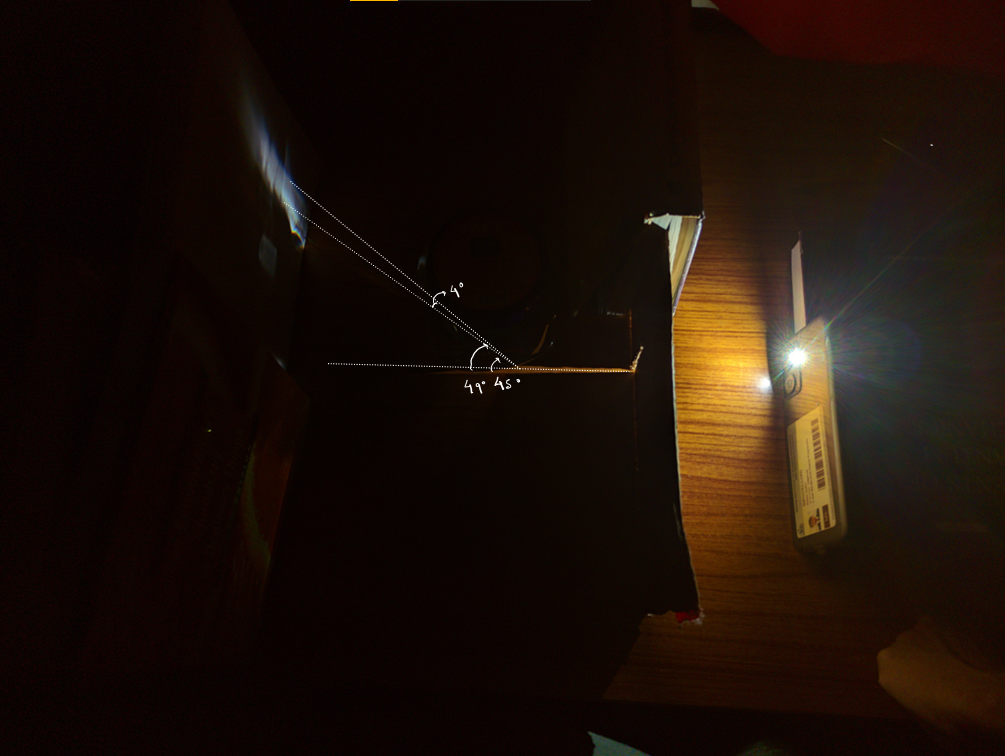
\includegraphics[scale =0.3]{red_violet.png}
        \caption{Measuring the angle of deviation for the red and violet lights.}
        \label{Measuring the angle of deviation for the red and violet lights}
    \end{figure}

\end{comment}
    
Now, with $A= 90\degree$, angle of deviation for red light $\delta_{red}= 45\degree$ and angle of deviation for red light $\delta_{blue} = 49 \degree$, we get,
\begin{equation}
    \label{red_refractive value}
    \mu_{red} = 1.306 
\end{equation}
\begin{equation}
    \label{violet_refractive value}
    \mu_{blue} =1.324 
\end{equation}
\subsection{Part 1.b: Measuring the Refractive Index from the Critical angle utilizing the Total Internal Reflection Phenomenon}
    \begin{figure}[H]
        \centering
        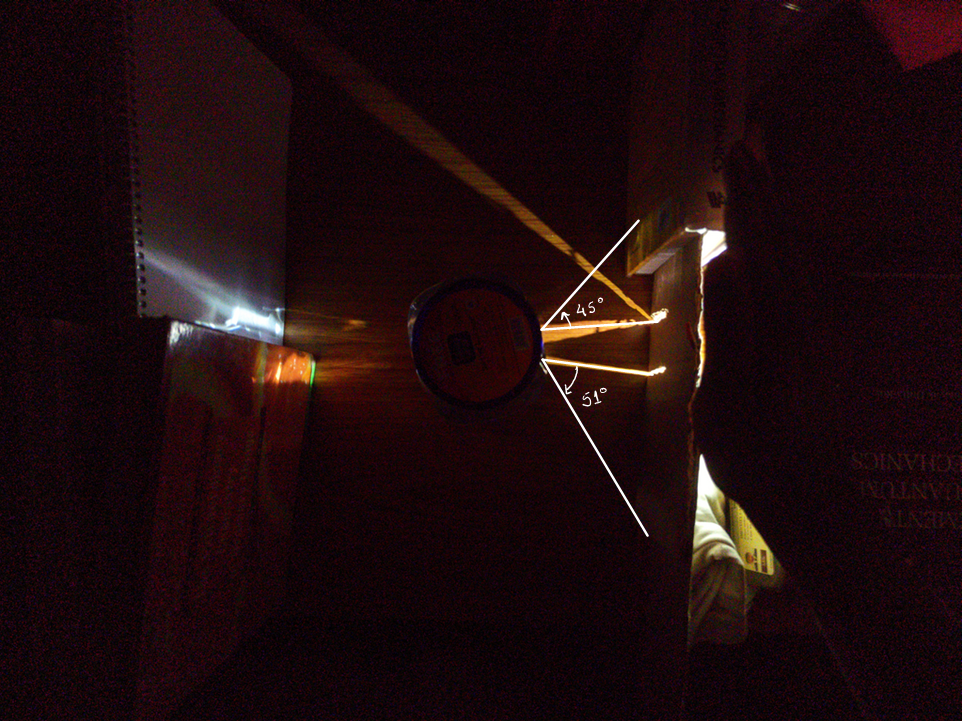
\includegraphics[scale =0.3]{TIR_double.png}
        \caption{Measuring the Critical angle}
        \label{Illustration of the Experimental procedure}
    \end{figure}
I tried it about 3 times, and all of them gave me different angles for the two surfaces with a $\SI{1}{\degree}$ variation and that must be due human error. In all, I decided to go with the average of the two i.e. $51\degree$ and $45\degree$ and that came to give the critical angle,
\begin{equation}
    \label{critical angle value}
    \theta_{critical} = 48 \degree
\end{equation}

Now knowing that,
\begin{equation}
    \label{critical angle relation with refractive index}
    \theta_{critical} = \sin{\frac{1}{\mu}}
\end{equation}
Here $\mu$ is the refractive index of the medium where light is going with respect to the medium from which the light is coming.
By utilizing \eqref{critical angle relation with refractive index} and putting \eqref{critical angle value}, we get,
\begin{equation}
    \label{Refractive index value using critical angle}
    {\mu_{water}}_{\theta_{critical}} = 1.346
\end{equation}


\begin{tcolorbox}[width=8cm,colback={aqua},title={NOTE: The Boundary of Conern},colbacktitle=white,coltitle=black]    
    Here, it has to be noted that the total internal reflection is happening at the water - plastic (refer to the qna section to understand why, and also see \href{https://drive.google.com/file/d/1LkRDtIguU656zTk9ufa4VYrhkumaocmM/view?usp=drive_link}{video} to visualize) boundary and that then from a optically rarer to a denser medium the light is traveling and so there the small plastic surface causes a shift which may result in the small errors that we are seeing in the final calculations.
\end{tcolorbox}

\subsection{Part 2: Understanding the discrepencies in the angle of the water prism}
\begin{figure}[H]
    \centering
    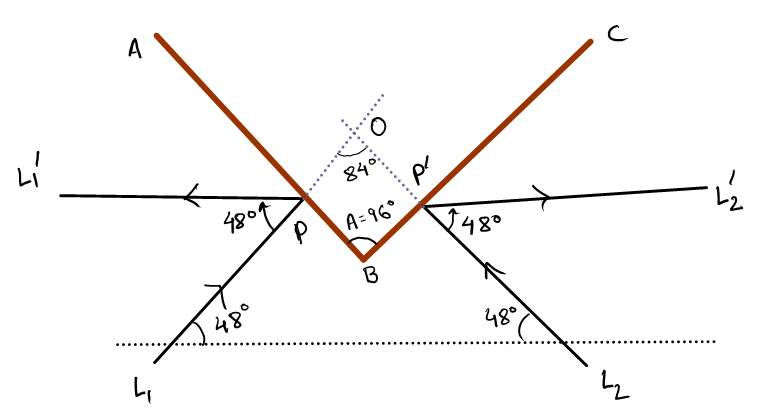
\includegraphics[scale =0.4]{Schematic diagram for prism angle.png}
    \caption{Schematic diagram for prism angle}
    \label{Schematic diagram for prism angle}
\end{figure}

I wasn't able to capture a picture of this stage as, I had to hold the whole setup at some height so that the angles just matched and then used the classical method of marking the spots while also taking into accound the height at which the apparatus was raised which was about 7cm above the desk.

From the schematic diagram, it is clear that
$\Delta L_1OL_2 $ using corresponding angles have $\angle OL_1L_2 \text{ and } \angle OL_2L_1 \text{ as } 48\degree $ and so using the properties of quadrilateral for $PBP'O$, we get

\begin{equation}
    \label{prism angle from light tir}
    A_{TIR} = 96\degree
\end{equation}
Note: I have used the average critical angle that I got instead of the two different data values.
\section{Analysis and Answering a few questions:}
\subsection{Where is the total internal reflection happening? At the Air-Plastic boundary or Plastic-Water boundary?}

Firstly, total internal reflection will not take place unless the incident light is traveling within the more optically dense medium towards the less optically dense medium.
\begin{enumerate}
  \item \textbf{Air to Plastic Interface}: As the light beam enters the plastic jar from air, it moves from a medium with a lower refractive index (air) to a higher refractive index (plastic). \textit{Total internal reflection is unlikely to occur at this interface} because the light is moving from a less optically dense medium to a more optically dense medium.

  \item \textbf{Plastic to Water Interface}: When the light beam enters the water inside the jar from the plastic, it moves from a higher refractive index medium (plastic) to a lower refractive index medium (water). If the angle of incidence at this interface is greater than the critical angle for the plastic-water boundary, total internal reflection could potentially occur here. This would result in the light being reflected back within the water.
  \\
  \textit{  Here, there is some thought process that can get involved. The assumption is that the plastic of the jar is optically more dense than water. Suppose, I don't know this fact then? I have the result that the total internal reflection is happening which is a fact. And I know that the air-plastic boundary is not the one for total internal reflection to occur. Henceforth, the only option remaining is the water-plastic boundary, and here, knowing that the phenomenon only happens when light travels from optically denser to rarer medium, we can surely say that the optical density of plastic is more than that of water. Meaning at the critical angle of water as the light enters through the plastic medium, it gets reflected back to plastic and them refracted back to the air medium.
}
\end{enumerate}

To summarize, as we know from the whole experimental results that total internal reflection is occurring in the setup of a plastic jar filled with water, \textbf{it's more likely to occur at the plastic-to-water interface}, where light moves from plastic (higher refractive index) to water (lower refractive index) at an angle of incidence greater than the critical angle for that interface.
\subsection{Why there are discrepancies regarding the presumed angle of prism and the real angle of prism and the calculated angle of prism?}

Let's first list the angles, 
Presumed angle, $A_{assumed} = 90\degree$,\\
Refer \eqref{Real angle of the prism} and \eqref{prism angle from light tir}, we have
$$A_{TIR} = 96\degree$$
$$A_{real} = 98 \degree$$
Here, we have different values and now let's do the reasoning.
\begin{enumerate}
    \item The Presumed angle was 90\degree and it's due to the fact that if I had obtained a perfect rectangular plastic box then it would have been true. But what I had was a bit bulky and even to the naked eyes clealy had more than 90 \degree at the edges.
    \item The real angle of the prism was 98\degree wih and error boundary of $\pm \SI{1}{\degree}$ and probably there are no questions about it as it is the physical structure of the jar.
    \item Now, from the calculations done to get the prism angle from the total internal reflection phenonmenon, we get the angle as 96\degree with again an error boundary of $\pm \SI{1}{\degree}$, and thus both the calculated values are actually the same if I consider that error has happened. 
    \item So, in all the discrepancies are only due to the fact that the jar that I used had clearly visible obtused angles at the edges and not rectangular as assumed. 
\end{enumerate}

\section{Extra Exploration}
\subsection{Salt water:}
I mixed about 20ml of common table salt\footnote{I also wanted to get it done using sugar, but totally forgot to get some from the canteen.} and knowing that Table salt has a density of 2.16g/cc \cite{Density_of_salt}, and so I added about 43.2 gram of salt in 500ml water. This created my salt-water prism, and here,
\begin{equation}
    \label{Critical angle salt}
    {\theta_{c}}_{salt} = 42 \degree
\end{equation}
So using \eqref{Critical angle salt} we get the refractive index of salt water as,
\begin{equation}
    \label{refractive salt}
    \mu_{salt_{water}} = 1.49
\end{equation}

\section{Error Analysis :}
\subsection{Instrumental/System Error}

From the \eqref{Deviationoflight}, then going by the usual process of taking the log of the expression and then differentiating while knowing that each error is additive,
\begin{equation}
    \label{the system error exp}
    \frac{\Delta \mu}{\mu} = \frac{\Delta \frac{\cos{\delta_{min}+A}}{2}}{\sin{\frac{\delta_{min}+A}{2}}} + \frac{\Delta \cos{\frac{A}{2}}}{\sin{\frac{A}{2}}}
\end{equation}
Now, using taylor expansion with only first term correction and also having a few approximations like the square of the errors being negligible, we can reduce the expression to,

\begin{equation}
    \label{sys error simplified}
    \frac{\Delta \mu}{\mu}= 2\frac{\Delta A}{A} + \frac{\Delta \delta_{min}}{\delta_{min}} + 
\end{equation}

Now, knowing that the error with regards to getting the angle of the light rays may atmost is $\pm 1 \degree$, we calculate the error for the refractive index for \eqref{Angle of deviation _45} and \eqref{prism angle from light tir}, we get,

\begin{equation}
    \label{Sys error calculated}
    \frac{\Delta \mu}{\mu} = 2 \frac{1\degree}{45\degree} + \frac{1 \degree}{96 \degree} = 0.032
\end{equation}
 So, according to \eqref{Sys error calculated}, the maximum error that I may have due to inaccurate measurements is 3.2\%.



\subsection{Relative Error analysis:}

$$\text{Relative Error \%} =$$
\begin{equation}
\label{Relative_Error}
\frac{|Observed Value-Literature Value|}{Literature Value} \times 100 \%
\end{equation}

I have calculated the value of the refractive index of water from various relations in this experiment, so calculating error for each of them should do the work. I thought of taking the average but then again the inside mechanism for each calculation uses a different optic property and so, I just left the errors untouched.
Also, I am going to be considering the refractive index of water (for yellow light) as the literature value (Refer \cite{refractive_index_water}) here.\\
For \eqref{Refractive Index from single setup}, we get,
$$\text{Relative Error \%}= 1.98\% $$

For \eqref{Refractive Index from single setup_real prism}, we get,
$$\text{Relative Error \%}= 5.47\% $$

For \eqref{Refractive index value using critical angle}, we get,
$$\text{Relative Error \%}= 0.97\%$$

The error values provide insight if there has been an occurrence of some error or human error, which is indeed the case for \eqref{Refractive index value using critical angle}, and that has mainly to do with the human error as getting it just right at the critical angle was very difficult due to the geometry of the jar that I used in this experiment. 
\\
\\ Also I wanted to check the value of the refractive index that I got for the red light and blue light for water, but I wasn't able to find some reliable sources to get the literature values. 


\section{Sources of Error:}
\begin{enumerate}
    \item \textbf{Systematic Error in Prism Angle}: The assumed prism angle ($A_{assumed} = 90\degree$) may introduce errors in calculations that depend on this angle. The actual prism angle ($A_{real}$) was measured to be $98\degree$, deviating from the assumption.
    

    \item \textbf{Human Error in Angle Measurement}: Manual angle measurements using a smartphone camera introduce the possibility of human error, such as parallax effects, inaccurate leveling, and imprecise readings.

    \item \textbf{Approximations in Calculations}: The simplifications and approximations made in calculations, such as neglecting the squares of error terms, can lead to inaccuracies in the final results.

    \item \textbf{Optical Aberrations}: The light passing through the plastic prism and water can experience optical aberrations, which might not be fully considered in the calculations.

    \item \textbf{Instrumental Errors}: Inaccuracies in the measuring instruments (ruler, protractor) and variations in the light source's intensity and stability can contribute to measurement errors.

    \item \textbf{Total Internal Reflection Boundary Assumption}: The assumption that total internal reflection occurs only at the plastic-water boundary may oversimplify the actual optical behavior, leading to discrepancies.

    \item \textbf{Surface Imperfections}: Scratches or irregularities on the surfaces of the plastic prism and container can alter the path of light and introduce errors.

    \item \textbf{Color Perception and Selection}: Subjective color selection from the spectrum for angle of deviation measurements introduces potential errors due to human perception.

    \item \textbf{Calibration of Smartphone Gyroscope}: The accuracy of using a smartphone gyroscope to level the camera with the experimental setup may affect the reliability of measurements.

    \item \textbf{Influence of Ambient Light}: Changes in ambient lighting conditions during the experiment can impact angle measurements and color selection.

    \item \textbf{Assumptions in Refractive Index Calculation}: Assumptions made in calculating refractive indices using different methods (critical angle, deviation of light) might not capture all complexities of the experiment.

\end{enumerate}

It is important to acknowledge these potential sources of error when interpreting the experimental results and considering the accuracy and reliability of calculated values.
\begin{tcolorbox}[width=8cm,colback={aqua},title={Note From The Author},colbacktitle=white,coltitle=black]    
    I was again checking the instructions and then I saw one criteria that you needed, that was the video to include me taking the measurements, but the video I provided had me setting the water jar/box up at the appropriate position. But, then again I used photographs only to get the accurate angles which were of concern. In short, the \href{https://drive.google.com/drive/folders/1HpE8DsCllbn2vvjRN1D8Pb3C0fbAIA9V?usp=sharing}{photographs} themselves were my measurements. Henceforth, the idea of the required video would not have made much sense.  
\end{tcolorbox}

\section{Conclusion and Inferences}
The experimental investigation focused on exploring light refraction and total internal reflection using a self-constructed water box prism apparatus. The findings and observations provide valuable insights into optical phenomena and experimental challenges:

\begin{enumerate}
    \item The refractive index of water was determined using two methods: minimum deviation and critical angle. The obtained values were $\mu_{water} = 1.306$ and $\mu_{water} = 1.346$, respectively, highlighting the importance of refractive index in light propagation.
    
    \item Total internal reflection was observed at the plastic-water interface, confirming the critical angle phenomenon. This underscores the role of refractive index mismatch in optical behaviors.
    
    \item Discrepancies in the prism angle were identified, with the actual angle measured as $98\degree$ compared to the assumed $90\degree$. This discrepancy led to errors in calculations, emphasizing the need for accurate measurements.
    
    \item The refractive index of saltwater was found to be $\mu_{salt_{water}} = 1.49$, illustrating how altering the medium influences light refraction.
    
    \item Error analysis revealed various sources of inaccuracies, including instrumental limitations, human measurement errors, and assumptions made during calculations.
    
    \item In conclusion, the experiment showcased the practical application of optical principles in a controlled setup. It demonstrated the complex interplay between light and matter, emphasizing the importance of precision and careful consideration of experimental factors.
    
    \item The study highlighted the challenges inherent in experimental design and data analysis, while also showcasing the potential for further exploration and learning in the field of optics.
\end{enumerate}

The experimental insights and outcomes contribute to a deeper understanding of light-matter interactions.

\bibliographystyle{abbrvurl}
\bibliography{ref}
\end{document}